% Chapter 1

\chapter{Introducción general} % Main chapter title

\label{Chapter1} % For referencing the chapter elsewhere, use \ref{Chapter1} 
\label{IntroGeneral}

%----------------------------------------------------------------------------------------

% Define some commands to keep the formatting separated from the content 
\newcommand{\keyword}[1]{\textbf{#1}}
\newcommand{\tabhead}[1]{\textbf{#1}}
\newcommand{\code}[1]{\texttt{#1}}
\newcommand{\file}[1]{\texttt{\bfseries#1}}
\newcommand{\option}[1]{\texttt{\itshape#1}}
\newcommand{\grados}{$^{\circ}$}

%----------------------------------------------------------------------------------------

%\section{Introducción}

%----------------------------------------------------------------------------------------
\section{Aprendiendo \LaTeX{}}

\LaTeX{} no es \textsc{WYSIWYG} (What You See is What You Get), a diferencia de los procesadores de texto como Microsoft Word o Pages de Apple o incluso LibreOffice en el mundo open-source. En lugar de ello, un documento escrito para \LaTeX{} es en realidad un archivo de texto simple o llano que \emph{no contiene formato} . Nosotros le decimos a \LaTeX{} cómo deseamos que se aplique el formato en el documento final escribiendo comandos simples entre el texto, por ejemplo, si quiero usar texto en itálicas para dar énfasis, escribo \verb|\it{texto}| y pongo el texto que quiero en itálicas entre medio de las llaves. Esto significa que \LaTeX{} es un lenguaje del tipo \enquote{mark-up}, muy parecido a HTML.

\subsection{Una introducción (no tan corta) a \LaTeX{}}

Si sos nuevo en \LaTeX{}, hay un muy buen libro electrónico - disponible gratuitamente en Internet como un archivo PDF - llamado, \enquote{A (not so short) Introduction to \LaTeX{}}. El título del libro es generalmente acortado a simplemente \emph{lshort}. Puede descargar la versión más reciente en inglés (ya que se actualiza de vez en cuando) desde aquí:
\url{http://www.ctan.org/tex-archive/info/lshort/english/lshort.pdf}

Se puede encontrar la versión en español en la lista en esta página: \url{http://www.ctan.org/tex-archive/info/lshort/}

\subsubsection{Una subsubsección}

Acá tiene un ejemplo de una ``subsubsección'' que es el cuarto nivel de ordenamiento del texto, después de capítulo, sección y subsección.  Como se puede ver, las subsubsecciones no van numeradas en el cuerpo del documento ni en el índice.  El formato está definido por la plantilla y no debe ser modificado.

\subsection{Guía matemática rápida para \LaTeX{}}

Si estás escribiendo un documento con mucho contenido matemático, entonces es posible que desees leer el documento de la AMS (American Mathematical Society) llamado, \enquote{A Short Math Guide for \LaTeX{}}. Se puede encontrar en línea en el siguiente link: \url{http://www.ams.org/tex/amslatex.html} en la sección \enquote{Additional Documentation} hacia la parte inferior de la página.


%----------------------------------------------------------------------------------------

\section{Utilizando esta plantilla}

Si estás familiarizado con \LaTeX{}, entonces podés explorar la estructura de directorios de esta plantilla y proceder a personalizarla agregando tu información en el bloque \emph{INFORMACIÓN DE LA PORTADA} en el archivo \file{memoria.tex}.  

Se puede continuar luego modificando el resto de los archivos siguiendo los lineamientos que se describen en la sección \ref{sec:FillingFile} en la página \pageref{sec:FillingFile}.

Debés asegurarte de leer el capítulo \ref{Chapter2} acerca de las convenciones utilizadas para las Memoria de los Trabajos Finales de la \degreename.

Si sos nuevo en \LaTeX{}, se recomienda que continúes leyendo el documento ya que contiene información básica para aprovechar el potencial de esta herramienta.


%----------------------------------------------------------------------------------------

\section{Qué incluye esta plantilla}

\subsection{Carpetas}

Esta plantilla se distribuye como una único archivo .zip que se puede descomprimir en varios archivos y carpetas. Asimismo, se puede consultar el repositorio git para obtener la última versión de los archivos, \url{https://github.com/patriciobos/Plantilla-CESE.git}. Los nombres de las carpetas son, o pretender ser, auto-explicativos.

\keyword{Appendices} -- Esta es la carpeta donde se deben poner los apéndices. Cada apéndice debe ir en su propio archivo \file{.tex}. Se incluye un ejemplo y una plantilla en la carpeta.

\keyword{Chapters} -- Esta es la carpeta donde se deben poner los capítulos de la memoria. Cada capítulo debe ir un su propio archivo \file{.tex} por separado.  Se ofrece por defecto, la siguiente estructura de capítulos y se recomienda su utilización dentro de lo posible:

\begin{itemize}
\item Capítulo 1: Introducción general	
\item Capítulo 2: Introducción específica
\item Capítulo 3: Diseño e implementación
\item Capítulo 4: Ensayos y resultados
\item Capítulo 5: Conclusiones

\end{itemize}

Esta estructura de capítulos es la que se recomienda para las memorias de la especialización.

\keyword{Figures} -- Esta carpeta contiene todas las figuras de la memoria.  Estas son las versiones finales de las imágenes que van a ser incluidas en la memoria.  Pueden ser imágenes en formato \textit{raster}\footnote{\url{https://en.wikipedia.org/wiki/Raster_graphics}} como \file{.png}, \file{.jpg} o en formato vectoriales\footnote{\url{https://en.wikipedia.org/wiki/Vector_graphics}} como \file{.pdf}, \file{.ps}.  Se debe notar que utilizar imágenes vectoriales disminuye notablemente el peso del documento final y acelera el tiempo de compilación por lo que es recomendable su utilización siempre que sea posible.

\subsection{Archivos}

También están incluidos varios archivos, la mayoría de ellos son de texto plano y se puede ver su contenido en un editor de texto. Después de la compilación inicial, se verá que más archivos auxiliares son creados por \ LaTeX{} o BibTeX, pero son de uso interno y no es necesario hacer nada en particular con ellos.  Toda la información necesaria para compilar el documento se encuentra en los archivos \file{.tex}, \file{.bib}, \file{.cls} y en las imágenes de la carpeta Figures.

\keyword{referencias.bib} - este es un archivo importante que contiene toda la información de referencias bibliográficas que se utilizarán para las citas en la memoria en conjunto con BibTeX. Usted puede escribir las entradas bibliográficas en forma manual, aunque existen también programas de gestión de referencias que facilitan la creación y gestión de las referencias y permiten exportarlas en formato BibTeX.  También hay disponibles sitios web como \url{books.google.com} que permiten obtener toda la información necesaria para una cita en formato BibTeX. Ver sección \ref{sec:biblio}

\keyword{MastersDoctoralThesis.cls} -- este es un archivo importante. Es el archivos con la clase que le informa a \LaTeX{} cómo debe dar formato a la memoria. El usuario de la plantilla no debería necesitar modificar nada de este archivo.

\keyword{memoria.pdf} -- esta es su memoria con una tipografía bellamente compuesta (en formato de archivo PDF) creado por \LaTeX{}. Se distribuye con la plantilla y después de compilar por primera vez sin hacer ningún cambio se debería obtener una versión idéntica a este documento.

\keyword{memoria.tex} -- este es un archivo importante. Este es el archivo que tiene que compilar \LaTeX{} para producir la memoria como un archivo PDF. Contiene un marco de trabajo y estructuras que le indican a \LaTeX{} cómo diagramar la memoria.  Está altamente comentado para que se pueda entender qué es lo que realiza cada línea de código y por qué está incluida en ese lugar.  En este archivo se debe completar la información personalizada de las primeras sección según se indica en la sección \ref{sec:FillingFile}.

Archivos que \emph{no} forman parte de la distribución de la plantilla pero que son generados por \LaTeX{} como archivos auxiliares necesarios para la producción de la memoria.pdf son:

\keyword{memoria.aux} -- este es un archivo auxiliar generado por \LaTeX{}, si se borra \LaTeX{} simplemente lo regenera cuando se compila el archivo principal \file{memoria.tex}.

\keyword{memoria.bbl} -- este es un archivo auxiliar generado por BibTeX, si se borra BibTeX simplemente lo regenera cuando se compila el archivo principal \file{memoria.tex}. Mientras que el archivo \file{.bib} contiene todas las referencias que hay, este archivo \file{.bbl} contine sólo las referencias que han sido citadas y se utiliza para la construcción de la bibiografía.

\keyword{memoria.blg} -- este es un archivo auxiliar generado por BibTeX, si se borra BibTeX simplemente lo regenera cuando se compila el archivo principal \file{memoria.tex}.

\keyword{memoria.lof} -- este es un archivo auxiliar generado por \LaTeX{}, si se borra \LaTeX{} simplemente lo regenera cuando se compila el archivo principal \file{memoria.tex}.  Le indica a \LaTeX{} cómo construir la sección \emph{Lista de Figuras}.
 
\keyword{memoria.log} --  este es un archivo auxiliar generado por \LaTeX{}, si se borra \LaTeX{} simplemente lo regenera cuando se compila el archivo principal \file{memoria.tex}. Contiene mensajes de \LaTeX{}. Si se reciben errores o advertencias durante la compilación, se guardan en este archivo \file{.log}.

\keyword{memoria.lot} -- este es un archivo auxiliar generado por \LaTeX{}, si se borra \LaTeX{} simplemente lo regenera cuando se compila el archivo principal \file{memoria.tex}.  Le indica a \LaTeX{} cómo construir la sección \emph{Lista de Tablas}.

\keyword{memoria.out} -- este es un archivo auxiliar generado por \LaTeX{}, si se borra \LaTeX{} simplemente lo regenera cuando se compila el archivo principal \file{memoria.tex}.

De esta larga lista de archivos, sólo aquellos con la extensión \file{.bib}, \file{.cls} y \file{.tex} son importantes.  Los otros archivos auxiliares pueden ser ignorados o borrados ya que \LaTeX{} y BibTeX los regenerarán durante la compilación.

%----------------------------------------------------------------------------------------

\section{Entorno de trabajo}

Ante de comenzar a editar la plantilla debemos tener un editor \LaTeX{} instalado en nuestra computadora.  En forma análoga a lo que sucede en lenguaje C, que se puede crear y editar código con casi cualquier editor, existen ciertos entornos de trabajo que nos pueden simplificar mucho la tarea.  En este sentido, se recomienda, sobre todo para los principiantes en \LaTeX{} la utilización de TexMaker, un programa gratuito y multi-plantaforma que está disponible tanto para windows como para sistemas GNU/linux.

La versión más reciente de TexMaker es la 4.5 y se puede descargar del siguiente link: \url{http://www.xm1math.net/texmaker/download.html}. Se puede consultar el manual de usuario en el siguiente link: \url{http://www.xm1math.net/texmaker/doc.html}.
 

\subsection{Paquetes adicionales}

Si bien durante el proceso de instalación de TexMaker, o cualquier otro editor que se haya elegido, se instalarán en el sistema los paquetes básicos necesarios para trabajar con \LaTeX{}, la plantilla de los trabajos de Especialización y Maestría requieren de paquete adicionales.

Se indican a continuación los comandos que se deben introducir en la consola de Ubuntu (ctrl + alt + t) para instalarlos:

\begin{lstlisting}[language=bash]
  $ sudo apt install texlive-lang-spanish texlive-science 
  $ sudo apt install texlive-bibtex-extra biber
  $ sudo apt install texlive texlive-fonts-recommended
  $ sudo apt install texlive-latex-extra
\end{lstlisting}


\subsection{Configurando TexMaker}
\label{subsec:configurando}



Una vez instalado el programa y los paquetes adicionales se debe abrir el archivo memoria.tex con el editor para ver una pantalla similar a la que se puede apreciar en la figura \ref{fig:texmaker}. 
Una vez instalado el programa y los paquetes adicionales se debe abrir el archivo memoria.tex con el editor para ver una pantalla similar a la que se puede apreciar en la figura \ref{fig:texmaker}. 
Una vez instalado el programa y los paquetes adicionales se debe abrir el archivo memoria.tex con el editor para ver una pantalla similar a la que se puede apreciar en la figura \ref{fig:texmaker}. 
Una vez instalado el programa y los paquetes adicionales se debe abrir el archivo memoria.tex con el editor para ver una pantalla similar a la que se puede apreciar en la figura \ref{fig:texmaker}. 

\vspace{1cm}

\begin{figure}[htbp]
	\centering
	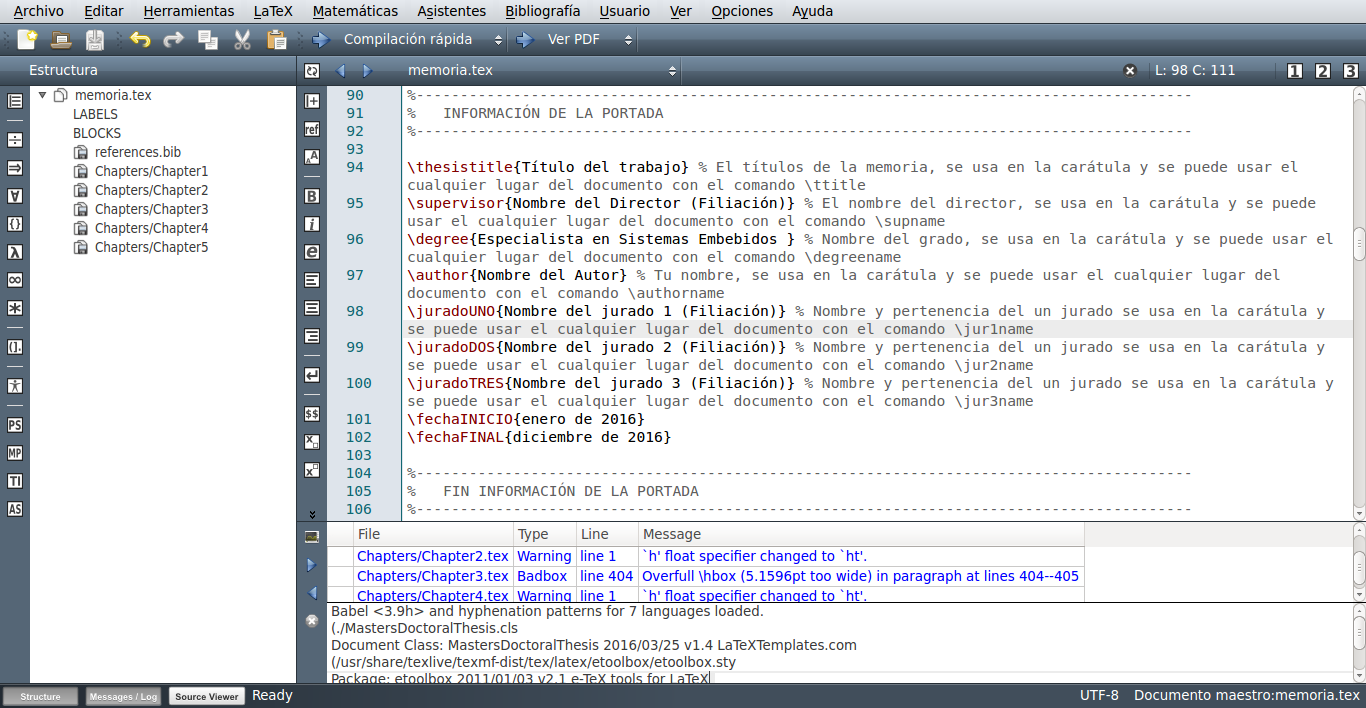
\includegraphics[width=.5\textwidth]{./Figures/texmaker.png}
	\caption{Entorno de trabajo de texMaker.}
	\label{fig:texmaker}
\end{figure}

\vspace{1cm}

Notar que existe una vista llamada Estructura a la izquierda de la interfaz que nos permite abrir desde dentro del programa los archivos individuales de los capítulos.  A la derecha se encuentra una vista con el archivo propiamente dicho para su edición. Hacia la parte inferior se encuentra una vista del log con información de los resultados de la compilación.  En esta última vista pueden aparecen advertencias o \textit{warning}, que normalmente pueden ser ignorados, y los errores que se indican en color rojo y deben resolverse para que se genere el PDF de salida.

Recordar que el archivo que se debe compilar con PDFLaTeX es \file{memoria.tex}, si se tratara de compilar alguno de los capítulos saldría un error.  Para salvar la molestia de tener que cambiar de archivo para compilar cada vez que se realice una modificación en un capítulo, se puede definir el archivo \file{memoria.tex} como ``documento maestro'' yendo al menú opciones -> ``definir documento actual como documento maestro'', lo que permite compilar con PDFLaTeX memoria.tex directamente desde cualquier archivo que se esté modificando . Se muestra esta opción en la figura \ref{fig:docMaestro}.

\begin{figure}[h]
	\centering
	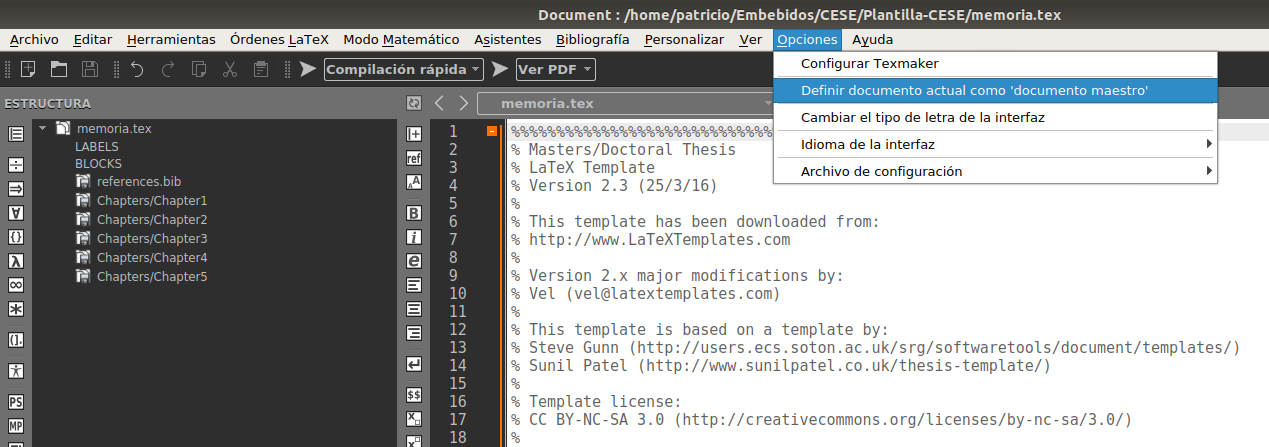
\includegraphics[width=\textwidth]{./Figures/docMaestro.png}
	\caption{Definir memoria.tex como documento maestro.}
	\label{fig:docMaestro}
\end{figure}

En el menú herramientas se encuentran las opciones de compilación.  Para producir un archivo PDF a partir de un archivo .tex se debe ejecutar PDFLaTeX (el shortcut es F6). Para incorporar nueva bibliografía se debe utilizar la opción BibTeX del mismo menú herramientas (el shortcut es F11).

Notar que para actualizar las tablas de contenidos se debe ejecutar PDFLaTeX dos veces.  Esto se debe a que es necesario actualizar algunos archivos auxiliares antes de obtener el resultado final.  En forma similar, para actualizar las referencias bibliográficas se debe ejecutar primero PDFLaTeX, después BibTeX y finalmente PDFLaTeX dos veces por idénticos motivos.

\section{Personalizando la plantilla, el archivo \file{memoria.tex}}
\label{sec:FillingFile}

Para personalizar la plantilla se debe incorporar la información propia en los distintos archivos \file{.tex}. 

Primero abrir \file{memoria.tex} con TexMaker (o el editor de su preferencia). Se debe ubicar dentro del archivo el bloque de código titulado \emph{INFORMACIÓN DE LA PORTADA} donde se deben incorporar los primeros datos personales con los que se construirá automáticamente la portada.


%----------------------------------------------------------------------------------------

\section{El código del archivo \file{memoria.tex} explicado}

El archivo \file{memoria.tex} contiene la estructura del documento y es el archivo de mayor jerarquía de la memoria.  Podría ser equiparable a la función \emph{main()} de un programa en C, o mejor dicho al archivo fuente .c donde se encuentra definida la función main().

La estructura básica de cualquier documento de \LaTeX{} comienza con la definición de clase del documento, es seguida por un preámbulo donde se pueden agregar funcionalidades con el uso de \texttt{paquetes} (equiparables a bibliotecas de C), y finalmente, termina con el cuerpo del documento, donde irá el contenido de la memoria.

\lstset{%
  basicstyle=\small\ttfamily,
  language=[LaTeX]{TeX}
}

\begin{lstlisting}
\documentclass{article}  <- Definicion de clase
\usepackage{listings}	 <- Preambulo

\begin{document}	 <- Comienzo del contenido propio 
	Hello world!
\end{document}
\end{lstlisting}


El archivo \file{memoria.tex} se encuentra densamente comentado para explicar qué páginas, secciones y elementos de formato está creando el código \LaTeX{} en cada línea. El código está dividido en bloques con nombres en mayúsculas para que resulte evidente qué es lo que hace esa porción de código en particular. Inicialmente puede parecer que hay mucho código \LaTeX{}, pero es principalmente código para dar formato a la memoria por lo que no requiere intervención del usuario de la plantilla.  Sí se deben personalizar con su información los bloques indicados como:

\begin{itemize}
	\item Informacion de la memoria
	\item Resumen
	\item Agradecimientos
	\item Dedicatoria
\end{itemize}

El índice de contenidos, las listas de figura de tablas se generan en forma automática y no requieren intervención ni edición manual por parte del usuario de la plantilla. 

En la parte final del documento se encuentran los capítulos y los apéndices.  Por defecto se incluyen los 5 capítulos propuestos que se encuentran en la carpeta /Chapters. Cada capítulo se debe escribir en un archivo .tex separado y se debe poner en la carpeta \emph{Chapters} con el nombre \file{Chapter1}, \file{Chapter2}, etc\ldots El código para incluir capítulos desde archivos externos se muestra a continuación.

\begin{verbatim}
	% Chapter 1

\chapter{Introducción general} % Main chapter title

En este capítulo se realiza una breve introducción a la necesidad que condujo al desarrollo del trabajo. Se presenta a los sistemas embebidos y el estado del arte de dispositivos similares. Asimismo, se explica el objetivo y los alcances del trabajo.

\label{Chapter1} % For referencing the chapter elsewhere, use \ref{Chapter1} 
\label{IntroGeneral}

%----------------------------------------------------------------------------------------

% Define some commands to keep the formatting separated from the content 
\newcommand{\keyword}[1]{\textbf{#1}}
\newcommand{\tabhead}[1]{\textbf{#1}}
\newcommand{\code}[1]{\texttt{#1}}
\newcommand{\file}[1]{\texttt{\bfseries#1}}
\newcommand{\option}[1]{\texttt{\itshape#1}}
\newcommand{\grados}{$^{\circ}$}

%----------------------------------------------------------------------------------------

%\section{Introducción}

%----------------------------------------------------------------------------------------
\section{Sistemas embebidos en la agricultura}

En las últimas décadas, la cosecha de kiwi ha experimentado un notable proceso de transformación, impulsado por la integración de tecnologías como los sistemas embebidos. Estos sistemas, capaces de realizar tareas específicas en tiempo real, se han vuelto fundamentales en la modernización de este sector.

Por otra parte, una de las actividades clave consiste en estimar, lo más exactamente posible, la producción total, ya que esto condiciona un conjunto importante de aspectos logísticos que deben ser atendidos correctamente durante la recolección.

Actualmente, el volumen de cosecha se estima al contar los frutos por unidad de superficie en una etapa avanzada de desarrollo. Sin embargo, esta evaluación tardía es demasiado cercana a la cosecha y muy dificultosa en plantaciones grandes.

Es en este contexto, que el prototipo KiwiScan permite recolectar imágenes de la plantación con el fin de realizar una detección de objetos. De esta forma, se obtiene una estimación de los frutos para facilitar la toma de decisiones operativas y estratégicas \citep{Mendoza2021}.

\subsection{Requerimientos del sistema}

Se detallan los requerimientos del sistema, con las funcionalidades y características necesarias para cumplir con los objetivos del proyecto.

\begin{enumerate}
	\item Requerimientos funcionales:
		\begin{enumerate}
			\item El sistema debe registrar la temperatura del ambiente.
			\item El sistema debe registrar la humedad del ambiente.
			\item El sistema debe informar el espacio disponible de la tarjeta microSD.
            \item El sistema debe informar la cantidad de fotos tomadas.
		\end{enumerate}
	\item Requerimientos no funcionales:
		\begin{enumerate}
			\item El sistema debe ser escalable, de forma de poder agregar más sensores en el futuro.
			\item El firmware debe estar modularizado.
            \item El firmware debe estar sobre un sistema operativo.
		\end{enumerate}
    \item Requerimientos de interfaz gráfica en la pantalla LCD:
		\begin{enumerate}
			\item Se debe mostrar los valores de humedad y temperatura.
			\item Se debe mostrar el espacio disponible en la tarjeta microSD.
            \item Se debe mostrar la cantidad de fotos tomadas.
            \item La información en pantalla debe actualizarse cada 5 segundos.
		\end{enumerate}
    \item Requerimientos de interoperabilidad:
		\begin{enumerate}
			\item Las fotos deben almacenarse en un formato de archivo JPG o JPEG.
			\item Las imágenes capturadas deben tener un mínimo de resolución de 640 x 480.
            \item Cada imagen guardada no debe superar los 10 MB.
		\end{enumerate}
    \item Requerimientos de documentación:
		\begin{enumerate}
			\item Todo el código fuente debe estar comentado.
			\item Se debe presentar un informe de avance del proyecto.
		\end{enumerate}
\end{enumerate}

%----------------------------------------------------------------------------------------

\section{Estado del arte}

Durante la etapa de investigación del trabajo, se realizó una búsqueda de productos comerciales en el mercado local e internacional. Se encontraron algunos con características similares al que se pretende desarrollar. Un dato interesante a resaltar es que todos los productos hallados provienen del mercado internacional; no se identificó ningún producto o empresa que ofrezca este tipo de soluciones en el mercado local hasta el momento. A continuación, se describen los hallazgos encontrados.

\subsection{Fruitometry}

La tecnología de estimación digital de cultivos (DCE) de Fruitometry que se muestra en la figura \ref{fig:Fruitometry}, permite a los productores y administradores de huertos observar el desempeño de su cultivo durante la temporada de cosecha. Esto ayuda a maximizar los rendimientos, reducir los costos de cultivo y proporcionar estimaciones antes de la recolección.

Las unidades de campo, montadas en cuatriciclos y vehículos todo terreno, contienen una variedad de cámaras y sensores que capturan información sobre la densidad de cultivos y las características del huerto. Para cada escaneo de la plantación, se toman miles de fotografías. Luego, estas se procesan en tiempo real mediante el motor de inteligencia artificial con aprendizaje profundo para identificar brotes, flores, frutos y características de interés.

Este conjunto de datos se utiliza para crear un mapa de calor de densidad resumido y generar informes que se usan para tomar decisiones sobre cómo mejorar el rendimiento del huerto, identificar áreas que requieren atención y dirigir la mano de obra hacia ellas \citep{WEBSITE:Fruitometry2024}.

\vspace{1cm}
\begin{figure}[htbp]
	\centering
	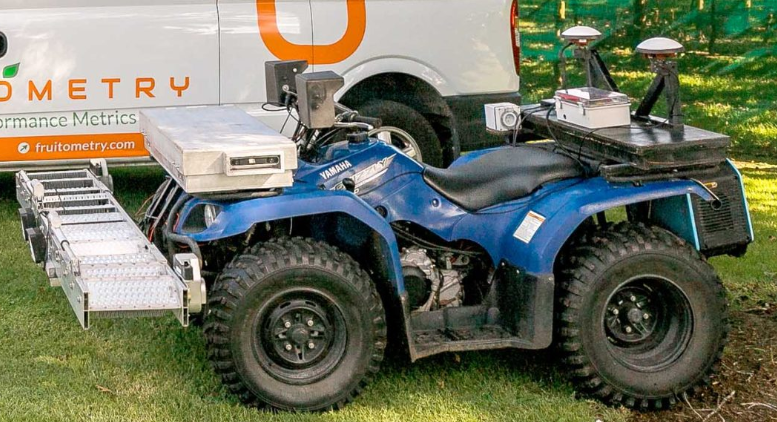
\includegraphics[width=.5\textwidth]{./Figures/Fruitometry.png}
	\caption{Unidad de campo Fruitometry\protect\footnotemark.}
	\label{fig:Fruitometry}
\end{figure}
\vspace{1cm}

\footnotetext{Imagen tomada de \url{https://fruitometry.com/about-fruitometry/}}

\subsection{Detección de kiwis en imágenes de campo}

En un trabajo de investigación realizado en la Universidad Yangling, China, se capturaron imágenes de kiwis en un huerto bajo diferentes condiciones de iluminación y en distintos momentos del día: mañana, tarde y noche, tanto con flash como sin él. Estas fotografías fueron empleadas para la detección de objetos mediante un modelo llamado Faster R-CNN, implementado con la arquitectura VGG16. Después de aplicar las detecciones, el modelo alcanzó una precisión promedio del 87,61 \%. En la figura \ref{fig:Song2019} se muestran los resultados obtenidos.

Este sistema de visión artificial resultó ser eficaz en la detección de diferentes categorías de frutos en el campo y actuó como un soporte fundamental al robot cosechador. Equipado con este sistema, el robot operó de manera continua durante la temporada de cosecha, lo que representó un avance significativo hacia la automatización de la recolección agrícola \citep{Song2019}.

\vspace{1cm}

\begin{figure}[htbp]
	\centering
	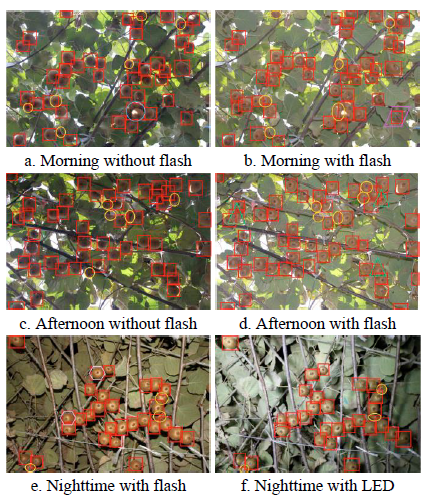
\includegraphics[width=.5\textwidth]{./Figures/Song2019.png}
	\caption{Resultados de una detección de objetos\protect\footnotemark.}
	\label{fig:Song2019}
\end{figure}

\vspace{1cm}
\footnotetext{Imagen tomada de "Kiwifruit detection in field
images using Faster R-CNN with VGG16"}

\newpage
\subsection{Calibrado de frutas}

Existen diversos productos comerciales que aplican la detección de objetos para llevar a cabo procesos de clasificación y calibrado de frutas u hortalizas. Estas máquinas, diseñadas específicamente para grandes cadenas de distribución, automatizan la selección y el empaquetado de los productos, lo que incrementa la eficiencia y reduce los tiempos operativos. El sistema funciona a través de una cinta transportadora equipada con cámaras, que capturan imágenes en tiempo real de cada elemento \citep{WEBSITE:Unitec2024}.

Además de identificar cada objeto, las cámaras registran una serie de parámetros importantes, como el diámetro, la longitud, la forma y, en algunos casos, el color. Estos datos se procesan con algoritmos de visión artificial, que clasifican los productos según criterios preestablecidos de calidad.

%----------------------------------------------------------------------------------------

\section{Objetivo y alcances}


En la siguiente sección se describen los objetivos del proyecto, los alcances y los aspectos no considerados en el desarrollo del prototipo.

\subsection{Objetivo}

El objetivo del presente trabajo es el desarrollo e implementación de un prototipo que permita contabilizar el rendimiento esperado de un lote de producción de kiwi en forma temprana, a través del procesamiento de imágenes.

\subsection{Alcances contemplados}
El alcance establecido para el trabajo incluyó las siguientes tareas:

\begin{itemize}
\item Implementación de un prototipo funcional que toma fotografías de forma automática.
\item Desarrollo del firmware sobre un sistema operativo de tiempo real.
\end{itemize}

\subsection{Aspectos no incluidos en el prototipo}

El alcance establecido para el trabajo no incluye las siguientes tareas:

\begin{itemize}
\item Desarrollo del modelo de detección de objetos.
\item Recolección de imágenes para el proceso de entrenamiento.
\item Pruebas de funcionamiento en la plantación.
\end{itemize}

%----------------------------------------------------------------------------------------

	\chapter{Introducción específica} % Main chapter title

\label{Chapter2}

%----------------------------------------------------------------------------------------
%	SECTION 1
%----------------------------------------------------------------------------------------
En el presente capítulo se describen los componentes de hardware, software y herramientas utilizados para realizar el trabajo.

\section{Estructura del sistema}

En las siguientes secciones se describe la estructura del sistema, con un enfoque en los sistemas embebidos, la detección de objetos y el prototipo KiwiScan.

\subsection{Los sistemas embebidos}

En el contexto de la agricultura moderna están diseñados para realizar tareas específicas y en tiempo real. En el caso de KiwiScan para la plantación de kiwi, el sistema se compone de una serie de módulos, como cámaras, sensores, pantallas y unidades de almacenamiento. Este podrá montarse en un medio de transporte adecuado a las características de la plantación, lo que permite la captura automatizada de imágenes de los frutos, así como el registro de datos ambientales relevantes durante el recorrido. Los datos recolectados se almacenan localmente en una tarjeta microSD.

\subsection{Detección de Objetos}

La detección de objetos es una técnica avanzada de visión por computadora que permite identificar y clasificar objetos en las imágenes. Esta tecnología, ha demostrado ser particularmente valiosa en el ámbito agrícola, donde la precisión en la estimación de la producción y la gestión eficiente de recursos son esenciales \citep{Lim2020}. 

Para que la detección de objetos funcione correctamente, se requiere de un conjunto de imágenes de entrada. Luego, estas son procesadas mediante algoritmos de visión por computadora. Estos algoritmos analizan las imágenes para identificar y contar los frutos \citep{Montiel2019}.

La detección de objetos se basa en técnicas avanzadas, como el análisis de imágenes y el aprendizaje automático, que permiten distinguir entre kiwis maduros, inmaduros y otros objetos presentes en la plantación.

\newpage

\subsection{El prototipo KiwiScan}

El prototipo desarrollado, a partir de ahora denominado KiwiScan, está conformado por tres partes esenciales que permiten llevar a cabo su labor. Estas son:
\begin{itemize}
\item El nodo sensor: esta es la parte física o hardware del sistema, utilizado para adquirir las imágenes de la plantación.
\item El firmware: este abarca la lógica del sistema y se encarga de la adquisición, procesamiento y la gestión del almacenamiento de datos. Puede funcionar sobre un sistema operativo de tiempo real o no.
\item El modelo de detección de objetos: este permite realizar la contabilización de los frutos encontrados en las imágenes proporcionadas como entrada.
\end{itemize}

\section{Componentes principales de hardware}

En esta sección se describen en detalle los componentes de hardware seleccionados para este trabajo, que resultaron clave para garantizar el funcionamiento adecuado del prototipo.

\subsection{Plataforma de desarrollo STM32 Nucleo-F429ZI}
\label{subsec:F429ZI}

La placa STM32 Nucleo-F429ZI, que se muestra en la figura \ref{fig:STM32-F429ZI}, posee un núcleo ARM Cortex-M4. Esta placa ofrece una plataforma flexible para desarrollar aplicaciones embebidas, con una amplia variedad de interfaces y periféricos, como ADC, DAC, GPIO, SPI, I2C, USART, entre otros. Además, cuenta con compatibilidad con los ecosistemas Arduino y ST Morpho, lo que facilita la expansión y el prototipado rápido. Es ideal para proyectos que requieren procesamiento en tiempo real, gestión de múltiples tareas y alto rendimiento \citep{WEBSITE:Itt2024}.

Características:
\begin{itemize}
\item STM32F429ZIT6 en paquete LQFP144.
\item CPU ARM® Cortex®-M4 de 32 bits con FPU.
\item Frecuencia máxima de CPU de 180 MHz.
\item VDD de 1,8 V a 3,6 V.
\item Flash de 2048 KB.
\item GPIO (114) con capacidad de interrupción externa.
\item Controlador DMA de 16 flujos con FIFO y compatibilidad con ráfagas.
\item Temporizador de control avanzado.
\item Temporizadores de uso general.
\item CAN 2.0B activo.
\item USB 2.0 OTG SA.
\item I2C.
\item SPI.
\item USART/UART.
\item EFS.
\item SDIO.
\item Generador aleatorio (TRNG para entropía HW).
\item Ethernet.
\end{itemize}

\begin{figure}[htbp]
	\centering
	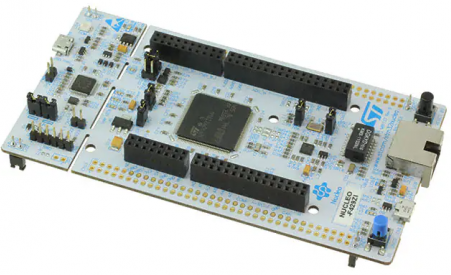
\includegraphics[width=.5\textwidth]{./Figures/STM32-F429ZI.png}
	\caption{Plataforma de desarrollo Nucleo-F429ZI\protect\footnotemark.}
	\label{fig:STM32-F429ZI}
\end{figure}

\footnotetext{Imagen tomada de \url{https://tienda.ityt.com.ar/plataforma-stm32/12702-nucleo-f429zi-stm32f429zi-stm32-cortex-m4-arm-itytarg.html}}

\subsection{Sensor de temperatura y humedad DHT11}
\label{subsec:dht11}

Este dispositivo, presentado en la figura \ref{fig:Dht11}, se utiliza para medir temperatura y humedad en ambientes controlados. Es altamente popular debido a su bajo costo y facilidad de uso. Dispone de un sensor capacitivo para medir la humedad y un termistor para la temperatura. El DHT11 proporciona lecturas de humedad en un rango del 20\% al 90\% con una precisión de ±5\%, y de temperatura entre 0 °C y 50 °C con una precisión de ±2 °C. Se comunica mediante una señal digital, lo que lo hace ideal para aplicaciones en sistemas embebidos y proyectos medianos \citep{WEBSITE:Dht112024}.

\begin{figure}[htbp]
	\centering
	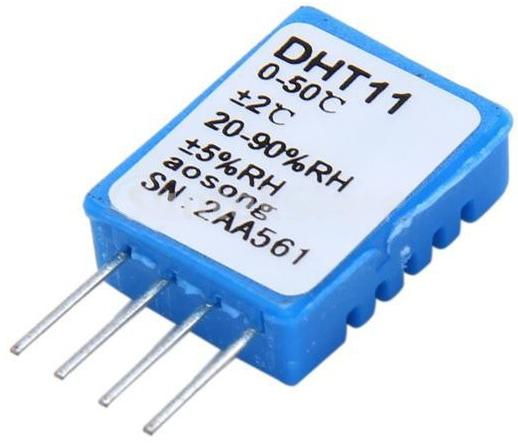
\includegraphics[width=.5\textwidth]{./Figures/dht11.png}
	\caption{Sensor de temperatura y humedad DHT11\protect\footnotemark.}
	\label{fig:Dht11}
\end{figure}

\footnotetext{Imagen tomada de \url{https://www.todomicro.com.ar/sensores/224-sensor-de-temperatura-y-humedad-dht11-arduino.html}}

\newpage

\subsection{Display LCD}
\label{subsec:DisplayLCD}

Esta pantalla, capaz de mostrar hasta 16 caracteres en 2 filas, se presenta en la figura \citep{WEBSITE:lcd2024}. Se utiliza en proyectos de electrónica y sistemas embebidos debido a su simplicidad y bajo costo. Cada carácter se forma a partir de una matriz de puntos de 5 x 8 píxeles, lo que permite visualizar letras, números y símbolos. El display es compatible con microcontroladores y microprocesadores, y se controla mediante interfaces paralelas o serie. Resulta ideal para mostrar información básica, como datos de sensores, mensajes o indicadores de estado en tiempo real \citep{WEBSITE:lcd2024}.

\begin{figure}[htbp]
	\centering
	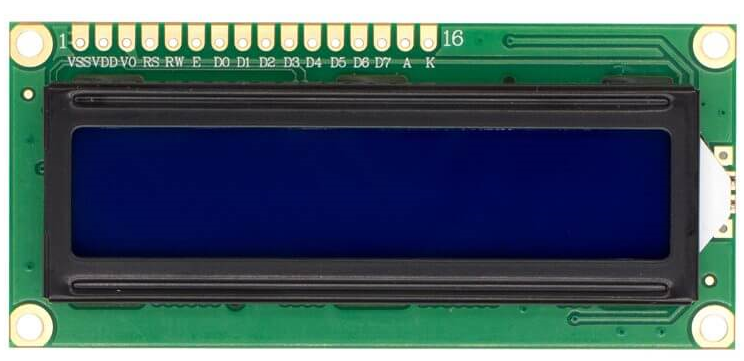
\includegraphics[width=.5\textwidth]{./Figures/lcd.png}
	\caption{Display LCD\protect\footnotemark.}
	\label{fig:lcd2024}
\end{figure}

\footnotetext{Imagen tomada de \url{https://uelectronics.com/producto/display-lcd-16x2-fondo-azul-amarillo/?srsltid=AfmBOorkJNNBhdEHSHGVr8xleeZYs_HXpCKmLdXyXVL5B2i6Fe4fKk0r}}

\subsection{Cámara Ov7670}
\label{subsec:camara}

Este módulo compacto de captura de imágenes, mostrado en la figura \ref{fig:camara2024}, se utiliza en proyectos de visión por computadora y sistemas embebidos. El sensor de imagen CMOS Ov7670 puede capturar imágenes en resolución VGA (640x480) y CIF (352x288), lo que lo hace adecuado para aplicaciones de procesamiento de imágenes, seguimiento de objetos y reconocimiento de patrones. La cámara se conecta a microcontroladores o plataformas de desarrollo como Arduino y STM32 mediante interfaces I2C o SCCB para configuración, y una interfaz de datos paralela para la transferencia de imágenes. Además, el módulo ofrece control automático de exposición, balance de blancos y eliminación de ruido, lo que garantiza imágenes de calidad en diversas condiciones de luz \citep{WEBSITE:camara2024}.

\begin{figure}[htbp]
	\centering
	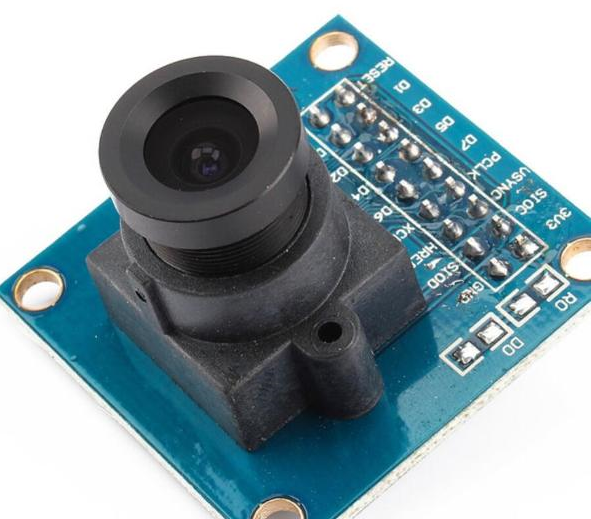
\includegraphics[width=.5\textwidth]{./Figures/camara.png}
	\caption{Cámara Ov7670\protect\footnotemark.}
	\label{fig:camara2024}
\end{figure}

\footnotetext{Imagen tomada de \url{https://www.arcaelectronica.com/products/modulo-de-camara-ov7670-arduino?srsltid=AfmBOopgmnm_0gtPYtNMaSrCGCOKnXMwbjdXpUfh84WJ_Hi9V3akPCPp}}

\subsection{Sensor ultrasónico HC-SR04}
\label{subsec:hcsr04}

Este dispositivo, mostrado en la figura \ref{fig:hcsr2024}, se utiliza para medir distancias con precisión en proyectos de robótica, sistemas embebidos y automatización. Emite ondas ultrasónicas que se reflejan en objetos cercanos y luego las capta el sensor. El tiempo que tarda la señal en regresar permite calcular la distancia al objeto. El HC-SR04 ofrece un rango de medición de 2 cm a 4 m, con una precisión de aproximadamente 3 mm. Se integra fácilmente con microcontroladores como Arduino o STM32 mediante un sistema de disparo y recepción de señal. Es ideal para aplicaciones como evitar obstáculos, medir niveles de líquido y sistemas de detección de proximidad \citep{WEBSITE:hcsr2024}.

\begin{figure}[htbp]
	\centering
	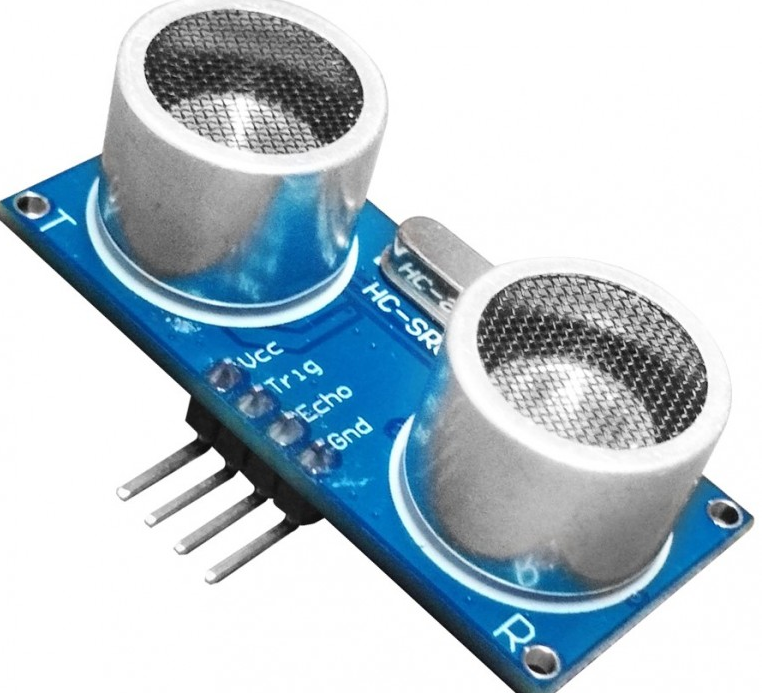
\includegraphics[width=.5\textwidth]{./Figures/hcsr04.png}
	\caption{Sensor ultrasónico HC-SR04\protect\footnotemark.}
	\label{fig:hcsr2024}
\end{figure}

\footnotetext{Imagen tomada de \url{https://www.todomicro.com.ar/modulos/81-sensor-ultrasonico-ultrasonido-hc-sr04-arduino-pic-robotica.html}}

\section{Herramientas de software y testing utilizados}

Las herramientas de software seleccionadas para este trabajo fueron fundamentales para el desarrollo y las pruebas del prototipo. A continuación se describen en detalle las características principales y los casos de uso de cada una.

\subsection{STM32 CubeIDE}
\label{subsec:stm32}

El sistema STM32 CubeIDE es un entorno de desarrollo integrado (IDE) creado por STMicroelectronics para trabajar con microcontroladores STM32. Basado en Eclipse, STM32 CubeIDE permite a los desarrolladores escribir, compilar y depurar código en lenguajes como C y C++ y por lo tanto facilita el desarrollo de aplicaciones embebidas. También integra herramientas como STM32CubeMX, que configura los periféricos del microcontrolador y genera código automáticamente. Estas  características contribuyen a reducir los errores y a acelerar el proceso de desarrollo. STM32 CubeIDE es compatible con sistemas operativos como Windows, macOS y Linux, y soporta una amplia gama de microcontroladores de la familia STM32, lo que lo convierte en una opción flexible para proyectos de sistemas embebidos \citep{WEBSITE:stm32}.

\subsection{Sistema operativo FreeRTOS}
\label{subsec:FreeRTOS}

Es un sistema operativo en tiempo real (RTOS) de código abierto, ampliamente utilizado en el desarrollo de aplicaciones embebidas. Diseñado para microcontroladores y sistemas de baja potencia, FreeRTOS ofrece un \textit{kernel} ligero y eficiente para gestionar tareas concurrentes de manera óptima. Soporta características clave como multitarea, gestión de memoria, sincronización entre tareas y temporización precisa, lo que lo convierte en una solución ideal para aplicaciones que requieren control preciso del tiempo y recursos limitados.

Además, FreeRTOS es compatible con una amplia variedad de arquitecturas de microcontroladores, incluidos los STM32. Cuenta con una extensa comunidad y soporte comercial a través de \textit{partners} como Amazon Web Services (AWS), que ofrece una versión ampliada llamada FreeRTOS IoT. Gracias a su escalabilidad y flexibilidad, FreeRTOS es una opción popular en proyectos que van desde dispositivos portátiles hasta sistemas industriales complejos \citep{WEBSITE:freertos}.

\subsection{Pruebas en CEEDLING}
\label{subsec:CEEDLING}

Es una herramienta de testing para proyectos en lenguaje C, diseñada para facilitar el desarrollo y la prueba de software embebido. Este marco de pruebas automatizado proporciona un entorno completo para la creación, ejecución y gestión de pruebas unitarias.

Ceedling integra varias herramientas esenciales para el testing, como CMock, un generador de mocks que simula dependencias y facilita el aislamiento de unidades de código durante las pruebas. Además, utiliza Unity, un framework de pruebas unitarias para C, que ofrece una serie de aserciones y macros para verificar el comportamiento del código.

La configuración y ejecución de pruebas con Ceedling se realizan a través de un archivo de configuración, lo que permite una integración fluida en el proceso de desarrollo. La herramienta soporta la ejecución de pruebas en diferentes entornos, genera informes detallados de cobertura de código y facilita la identificación de errores y defectos en el software \citep{WEBSITE:CEEDLING}.

\section{Protocolos de comunicación}

Los protocolos de comunicación seleccionados son esenciales para la interacción entre los diferentes componentes del sistema. UART permite la transmisión y recepción de datos de manera eficiente, lo que facilita la conexión entre microcontroladores y dispositivos periféricos.

I2C, por otra parte, ofrece una solución versátil para la comunicación entre múltiples dispositivos en el sistema. Su capacidad para identificar dispositivos mediante direcciones únicas garantiza una integración efectiva de sensores y otros periféricos, y de esta manera contribuye a optimizar la funcionalidad del prototipo.

\subsection{El protocolo UART}
\label{subsec:UART}

Es un protocolo de comunicación serial utilizado en sistemas embebidos y en la comunicación entre dispositivos electrónicos. UART permite la transmisión y recepción de datos en serie, es decir, un bit a la vez, a través de un solo canal de comunicación.

El funcionamiento de UART se basa en una comunicación asíncrona, lo que significa que no requiere una señal de reloj compartida entre los dispositivos que se comunican. En su lugar, utiliza parámetros de configuración como la velocidad de transmisión (\textit{baud rate}), la paridad, el número de bits de datos y el número de bits de parada para sincronizar la transmisión y recepción de datos. En la práctica, UART se emplea para conectar microcontroladores, módulos de comunicación, sensores y otros dispositivos electrónicos, lo que facilita la transferencia de datos \citep{WEBSITE:uart}. 

\subsection{El protocolo I2C}
\label{subsec:I2C}

Es un protocolo de comunicación serial ampliamente utilizado para conectar dispositivos en sistemas embebidos. Desarrollado por Philips Semiconductors (ahora NXP), I2C facilita la comunicación entre microcontroladores, sensores, memorias y otros periféricos mediante una interfaz de dos hilos.

El protocolo I2C utiliza dos líneas para la transmisión de datos: la línea de reloj (SCL) y la línea de datos (SDA). La línea SCL sincroniza la comunicación mediante la señal de reloj, mientras que la línea SDA transporta los datos entre los dispositivos conectados. Ambos hilos son bidireccionales, lo que permite que tanto el maestro como el esclavo envíen y reciban información.

I2C permite la comunicación en un bus que puede conectar múltiples dispositivos mediante una sola pareja de líneas. Cada dispositivo en el bus I2C tiene una dirección única que permite su identificación. Su implementación en sistemas embebidos abarca aplicaciones como la comunicación con sensores, controladores de pantallas y dispositivos de almacenamiento \citep{WEBSITE:i2c}.
 
	\chapter{Diseño e implementación} % Main chapter title

\label{Chapter3} % Change X to a consecutive number; for referencing this chapter elsewhere, use \ref{ChapterX}

\definecolor{mygreen}{rgb}{0,0.6,0}
\definecolor{mygray}{rgb}{0.5,0.5,0.5}
\definecolor{mymauve}{rgb}{0.58,0,0.82}

%%%%%%%%%%%%%%%%%%%%%%%%%%%%%%%%%%%%%%%%%%%%%%%%%%%%%%%%%%%%%%%%%%%%%%%%%%%%%
% parámetros para configurar el formato del código en los entornos lstlisting
%%%%%%%%%%%%%%%%%%%%%%%%%%%%%%%%%%%%%%%%%%%%%%%%%%%%%%%%%%%%%%%%%%%%%%%%%%%%%
\lstset{ %
  backgroundcolor=\color{white},   % choose the background color; you must add \usepackage{color} or \usepackage{xcolor}
  basicstyle=\footnotesize,        % the size of the fonts that are used for the code
  breakatwhitespace=false,         % sets if automatic breaks should only happen at whitespace
  breaklines=true,                 % sets automatic line breaking
  captionpos=b,                    % sets the caption-position to bottom
  commentstyle=\color{mygreen},    % comment style
  deletekeywords={...},            % if you want to delete keywords from the given language
  %escapeinside={\%*}{*)},          % if you want to add LaTeX within your code
  %extendedchars=true,              % lets you use non-ASCII characters; for 8-bits encodings only, does not work with UTF-8
  %frame=single,	                % adds a frame around the code
  keepspaces=true,                 % keeps spaces in text, useful for keeping indentation of code (possibly needs columns=flexible)
  keywordstyle=\color{blue},       % keyword style
  language=[ANSI]C,                % the language of the code
  %otherkeywords={*,...},           % if you want to add more keywords to the set
  numbers=left,                    % where to put the line-numbers; possible values are (none, left, right)
  numbersep=5pt,                   % how far the line-numbers are from the code
  numberstyle=\tiny\color{mygray}, % the style that is used for the line-numbers
  rulecolor=\color{black},         % if not set, the frame-color may be changed on line-breaks within not-black text (e.g. comments (green here))
  showspaces=false,                % show spaces everywhere adding particular underscores; it overrides 'showstringspaces'
  showstringspaces=false,          % underline spaces within strings only
  showtabs=false,                  % show tabs within strings adding particular underscores
  stepnumber=1,                    % the step between two line-numbers. If it's 1, each line will be numbered
  stringstyle=\color{mymauve},     % string literal style
  tabsize=2,	                   % sets default tabsize to 2 spaces
  title=\lstname,                  % show the filename of files included with \lstinputlisting; also try caption instead of title
  morecomment=[s]{/*}{*/}
}


%----------------------------------------------------------------------------------------
%	SECTION 1
%----------------------------------------------------------------------------------------
\section{Análisis del software}
 
La idea de esta sección es resaltar los problemas encontrados, los criterios utilizados y la justificación de las decisiones que se hayan tomado.






	% Chapter Template

\chapter{Ensayos y resultados} % Main chapter title

\label{Chapter4} % Change X to a consecutive number; for referencing this chapter elsewhere, use \ref{ChapterX}

En este capítulo se describen las pruebas realizadas para validar el hardware y el firmware desarrollados. Con el objetivo de verificar la precisión y robustez del sistema, se utilizaron herramientas de automatización de pruebas y hardware externo que permitieron contrastar y analizar los datos capturados por cada sensor. Estas pruebas revelaron el rendimiento del sistema y evaluaron el cumplimiento de los requisitos establecidos por cada módulo.

%----------------------------------------------------------------------------------------
%	SECTION 1
%----------------------------------------------------------------------------------------

\section{Pruebas unitarias del firmware}
\label{sec:pruebas_unitarias}

En esta sección se presentan pruebas unitarias para validar las funcionalidades clave del software, lo que asegura la precisión y estabilidad de cada componente. Durante la implementación de los drivers, se aplicó la metodología de desarrollo Test-Driven Development (TDD) \citep{ieee2023}, que establece la creación de pruebas unitarias antes de cada módulo y garantiza que el código cumpla con los requerimientos especificados desde las primeras etapas. Esta metodología permitió identificar errores y realizar ajustes con anticipación, optimizando la calidad del software. Para el desarrollo de pruebas automáticas, se empleó Ceedling, una herramienta robusta que facilitó la creación, ejecución y gestión de pruebas, asegurando una verificación consistente de cada funcionalidad.

\subsection{Prueba del sensor DHT11}
Para validar la implementación del driver del sensor DHT11, se emplearon informes de cobertura generados por Ceedling. Esta metodología no solo verificó la correcta adquisición de datos de temperatura y humedad, sino que también permitió evaluar la cobertura de las pruebas.

El reporte del código fue fundamental para identificar áreas del driver que no estaban cubiertas por las pruebas iniciales, lo que permitió realizar ajustes y optimizaciones en el código para asegurar una validación exhaustiva. Además, los resúmenes de resultados generados en consola ofrecieron una vista rápida y clara del desempeño de las pruebas.

\newpage

La cobertura obtenida mediante estas pruebas unitarias aseguró que el firmware estuviera preparado para manejar situaciones como valores atípicos o desconexiones inesperadas del sensor. Así, el proceso de validación del driver del DHT11 proporcionó no solo datos sobre el rendimiento y la cobertura del código, sino que también contribuyó a mejorar la confiabilidad y precisión del sistema en su conjunto. En la figura \ref{fig:test_sensor_dht11} se presentan los resultados de la prueba realizada.

\vspace{1cm}

\begin{figure}[htbp]
	\centering
	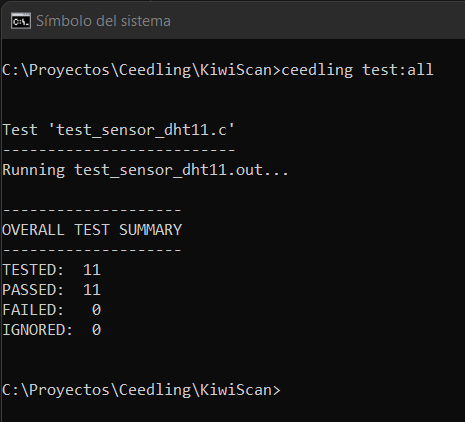
\includegraphics[width=0.7\textwidth, height=0.3\textheight]{./Figures/test_sensor_dht11.png}
	\caption{Test realizado al driver DHT11.}
	\label{fig:test_sensor_dht11}
\end{figure}

\vspace{1cm}

\subsection{Prueba del display LCD}

El driver del display LCD cumplió con múltiples requisitos, incluyendo la visualización de datos en tiempo real, cantidad de capturas tomadas, distancia del objetivo y alertas generadas, sin afectar el desempeño general del sistema. Ceedling proporcionó un resumen detallado de las métricas de prueba, que reflejó la cantidad de casos exitosos y fallidos, así como la cobertura de cada función en el driver.

Las pruebas revelaron detalles específicos sobre la interacción con el hardware, como la capacidad de la pantalla para responder a comandos de refresco rápido. En particular, los informes de cobertura destacaron áreas del driver con potencial de optimización, como la gestión de excepciones ante fallos de comunicación con el display. Esta observación motivó mejoras en la codificación del driver, fortaleciendo la detección y manejo de errores y, con ello, asegurando que el display muestre la información correcta.

Además, se validaron las capacidades del driver para recibir y mostrar correctamente la información generada por otros módulos, como los datos de los sensores de temperatura y humedad, el lector de tarjetas SD y el de distancia. Los resultados se presentan en la figura \ref{fig:test_lcd_display}.

\vspace{1cm}

\begin{figure}[htbp]
	\centering
	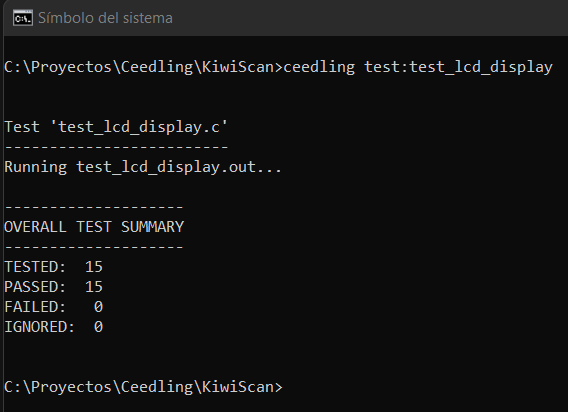
\includegraphics[width=0.7\textwidth, height=0.3\textheight]{./Figures/test_lcd_display.png}
	\caption{Test realizado al display LCD.}
	\label{fig:test_lcd_display}
\end{figure}

\vspace{1cm}

\subsection{Prueba de cámara Ov7670}

La validación del driver de la cámara Ov7670 fue fundamental para garantizar que el sistema capturara imágenes con precisión y fiabilidad, cumpliendo los requisitos en términos de resolución y capacidad de captura en tiempo real.

La prueba incluyó aspectos clave, como la inicialización de la cámara, la captura de imágenes en diferentes resoluciones y la transmisión de datos al proceso principal para su almacenamiento y análisis.

Durante las pruebas, se evaluaron distintas configuraciones de la cámara Ov7670, verificando los ajustes de resolución y formato de imagen. La cobertura obtenida en las pruebas reflejó la capacidad del driver para mantener la estabilidad y calidad en la captura de imágenes incluso en condiciones de carga intensa. Además, los informes de prueba permitieron identificar y solucionar fallas menores, como errores en la sincronización del módulo de captura o posibles pérdidas de datos en resoluciones altas, asegurando un flujo constante y sin interrupciones. La figura \ref{fig:test_ov7670_camera}
muestra los resultados de las pruebas realizadas.

Otro aspecto evaluado fue la integración del driver con el sistema general, garantizando que las imágenes capturadas por la cámara se transfirieran correctamente a los módulos de procesamiento y almacenamiento sin afectar el rendimiento del firmware. Este proceso resultó crucial para validar la robustez del sistema ante interrupciones inesperadas, verificando que el driver de la cámara mantuviera estabilidad y asegurará la disponibilidad de imágenes para el procesamiento posterior.

\vspace{1cm}

\begin{figure}[htbp]
	\centering
	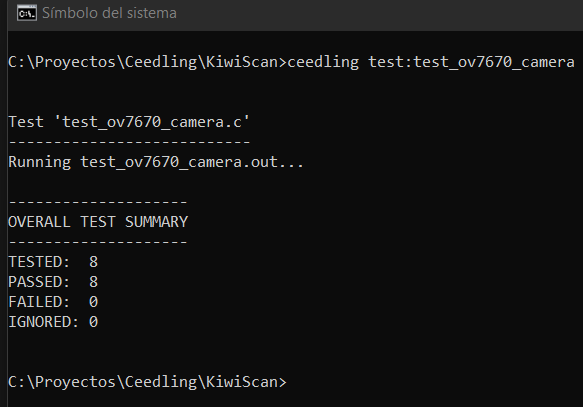
\includegraphics[width=0.7\textwidth, height=0.3\textheight]{./Figures/test_ov7670_camera.png}
	\caption{Test realizado a la cámara Ov7670.}
	\label{fig:test_ov7670_camera}
\end{figure}

\vspace{1cm}

\subsection{Prueba del sensor ultrasónico HC-SR04}

El proceso de prueba abarcó varias funciones clave del driver, incluyendo la inicialización del sensor, el envío de pulsos de activación, y la recepción y procesamiento de los ecos de respuesta que miden la distancia. Ceedling ejecutó pruebas unitarias para cada una de estas funciones, generando informes detallados sobre la precisión y consistencia de los resultados. Este enfoque garantizó que el sensor ofreciera mediciones confiables y respondiera adecuadamente ante diferentes distancias, desde rangos cortos hasta los límites efectivos del sensor.

Otra área de prueba clave fue la integración del sensor con el sistema general y la manera en que el driver del HC-SR04 gestionaba las interrupciones durante la medición de distancias. Esta verificación fue esencial para confirmar que el sistema mantuviera un flujo de datos continuo, entregando información precisa en tiempo real al módulo de procesamiento.

Finalmente, se realizaron pruebas para analizar el manejo de errores en el driver, especialmente en situaciones en las que el sensor no recibía respuesta de eco o detectaba obstrucciones inesperadas. Se validó que el sistema reaccionara correctamente ante estas situaciones, registrando la falta de datos o enviando alertas al proceso de alarmas cuando fuera necesario. La figura \ref{fig:test_hc_sr04_sensor} muestra los resultados de las pruebas realizadas.

\newpage

\vspace{1cm}

\begin{figure}[htbp]
	\centering
	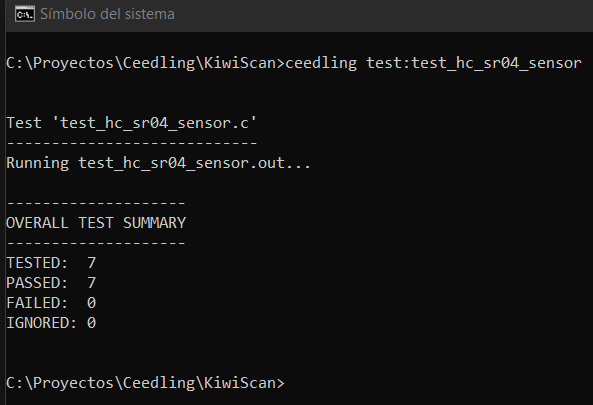
\includegraphics[width=0.7\textwidth, height=0.3\textheight]{./Figures/test_hc_sr04_sensor.png}
	\caption{Test realizado al sensor ultrasónico HC-SR04.}
	\label{fig:test_hc_sr04_sensor}
\end{figure}

\vspace{1cm}

\subsection{Prueba del lector de tarjetas SD}

Las pruebas iniciales evaluaron las operaciones de escritura y lectura, funciones esenciales para el almacenamiento continuo de datos capturados por los sensores. Cada operación fue probada con diferentes tamaños de archivos, simulando diversos escenarios de uso, desde pequeñas cantidades de datos hasta archivos de mayor tamaño, para determinar la capacidad del driver para manejar un flujo de datos sostenido.

Otro aspecto clave de las pruebas fue la verificación de la funcionalidad de borrado y la gestión del espacio disponible en la tarjeta SD. Se comprobó que el driver eliminaba datos de forma efectiva y detectaba con la cantidad de espacio liberado y restante tras cada operación.

Además, se evaluaron las capacidades del driver para detectar y gestionar tarjetas SD con diferentes formatos. La lectura y escritura en tarjetas formateadas en sistemas FAT32 y exFAT permitió verificar la flexibilidad del driver y su compatibilidad con distintos tipos de almacenamiento. Este aspecto fue crítico, pues garantiza que el sistema se adapte a diversas tarjetas sin requerir reconfiguraciones manuales.

Se simularon problemas comunes, como la extracción inesperada de la tarjeta, errores en la escritura y fallos de inicialización. Esto permitió observar cómo el driver respondía ante estos fallos, verificando que el sistema registrará la interrupción o emitiera alertas adecuadas sin comprometer la estabilidad del sistema. La figura \ref{fig:test_sd_card_reader} muestra los resultados de las pruebas realizadas.

\vspace{1cm}

\begin{figure}[htbp]
	\centering
	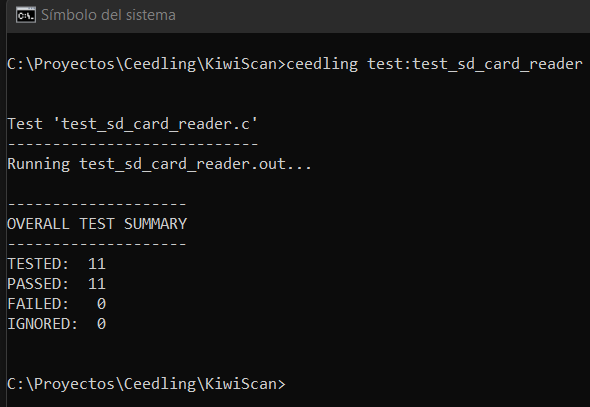
\includegraphics[width=0.7\textwidth, height=0.3\textheight]{./Figures/test_sd_card_reader.png}
	\caption{Test realizado al lector de tarjetas SD.}
	\label{fig:test_sd_card_reader}
\end{figure}

\vspace{1cm}

\subsection{Prueba de integración de drivers}

La prueba de integración de drivers tuvo como objetivo evaluar el desempeño conjunto de los componentes desarrollados y comprobar su funcionamiento de manera coordinada y sin interferencias. Esta prueba incluyó los drivers del sensor de temperatura y humedad DHT11, el sensor ultrasónico HC-SR04, la cámara OV7670, el display LCD y el lector de tarjetas SD, los cuales operaron simultáneamente para asegurar una respuesta del sistema.

En el proceso, cada driver fue evaluado en condiciones similares a las de su operación final, verificando la capacidad del sistema para gestionar la entrada y salida de datos sin fallas, interferencias ni retrasos perceptibles en los tiempos de respuesta. Los resultados indicaron que todos los drivers se integraron correctamente, funcionando sin dificultades en los ensayos realizados, con una sincronización adecuada entre los distintos módulos. La figura \ref{fig:test_integrated_drivers} muestra los resultados obtenidos.

Las pruebas confirmaron que el sistema responde adecuadamente a las demandas de funcionamiento en conjunto, sin comprometer la velocidad ni la precisión de las mediciones y salidas visuales.

\newpage

\vspace{1cm}

\begin{figure}[htbp]
	\centering
	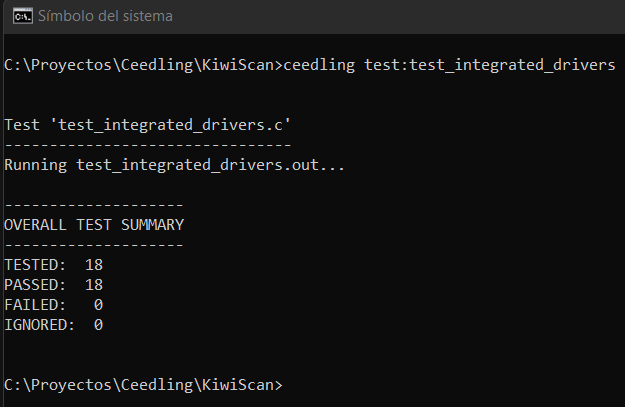
\includegraphics[width=0.7\textwidth, height=0.3\textheight]{./Figures/test_integrated_drivers.png}
	\caption{Test de integración de drivers.}
	\label{fig:test_integrated_drivers}
\end{figure}

\vspace{1cm}

\section{Pruebas funcionales del hardware}
\label{pruebas_funcionales_hardware}

Esta sección expone los ensayos realizados para evaluar la precisión y confiabilidad de los sensores integrados en el sistema. El propósito principal es contrastar las mediciones del sensor de temperatura y humedad DHT11, el sensor ultrasónico HC-SR04 y la cámara Ov7670 con las obtenidas por otros dispositivos o herramientas.

\subsection{Evaluación de precisión en temperatura y humedad del sensor DHT11}

Para determinar la precisión del sensor DHT11 en la medición de temperatura y humedad, se realizaron pruebas comparativas utilizando un termómetro higrómetro de laboratorio como referencia. Esta prueba tuvo lugar durante un periodo de dos horas, con mediciones cada 15 minutos a partir del mediodía. La prueba se llevó a cabo en un entorno controlado, con una temperatura base aproximada de 25 ° C, en horario de verano.

En cada intervalo de tiempo, se registraron los datos de temperatura y humedad captados por ambos dispositivos, lo que permitió identificar las diferencias entre el sensor DHT11 y el termómetro higrómetro. Se observó que el DHT11 reportó variaciones de entre 1 y 2 puntos respecto a la referencia de laboratorio, tanto en temperatura como en humedad, lo que muestra una desviación mínima. Los resultados de esta comparación se presentan en la tabla \ref{tab:DHT11_comparacion}.

\newpage

\begin{table}[h]
    \centering
    \caption[Comparación de mediciones de temperatura y humedad]{Comparación de mediciones de temperatura y humedad.}
    \begin{tabularx}{\textwidth}{l X X X X X X X}  % Cambia el ancho de la última columna
        \toprule
        \textbf{Hora} & \textbf{Temp. DHT11} & \textbf{Temp. higrómetro} & \textbf{Dif. temp.} & \textbf{Hum. DHT11} & \textbf{Hum. higrómetro} & \textbf{Dif. hum.} \\
        \midrule
        12:00 PM & 25.5 & 25.0 & +0.5 & 47 & 49 & -2\\		
        12:15 PM & 26.0 & 25.5 & +0.5 & 46 & 48	& -2\\
        12:30 PM & 26.3 & 26.0 & +0.3 & 48 & 49 & -1\\
        12:45 PM & 26.5 & 26.2 & +0.3 & 49 & 50 & -1\\
        01:00 PM & 26.7 & 26.5 & +0.2 & 50 & 52 & -2\\
        01:15 PM & 27.0 & 26.8 & +0.2 & 51 & 53 & -2\\
        01:30 PM & 27.2 & 27.0 & +0.2 & 52 & 54 & -2\\
        01:45 PM & 27.3 & 27.1 & +0.2 & 52 & 54 & -2\\
        02:00 PM & 27.5 & 27.3 & +0.2 & 53 & 55 & -2\\
        \bottomrule
    \end{tabularx}
    \label{tab:DHT11_comparacion}
\end{table}

\subsection{Análisis de precisión en medición de distancia con el sensor ultrasónico HC-SR04}

El objetivo de esta prueba fue evaluar la precisión del sensor ultrasónico HC-SR04 en la medición de distancias. Se establecieron seis puntos de referencia a distintas distancias de una muestra de una planta de kiwi: 50 centímetros, 1 metro, 1.5 metros, 2 metros, 2.5 metros y 3 metros. Las mediciones de referencia se obtuvieron con una cinta métrica convencional, y luego se registraron las lecturas del sensor HC-SR04 para cada posición.

Los resultados evidencian que el sensor HC-SR04 presenta una gran precisión en distancias cortas, detectando sin errores la medida de 50 centímetros. Sin embargo, conforme aumenta la distancia, se observan diferencias leves que van de 1 a 5 centímetros en comparación con la referencia. Estos datos demuestran que el sensor es bastante preciso en rangos de hasta un metro y mantiene una tolerancia aceptable para aplicaciones de detección de distancias mayores. La tabla \ref{tab:HCSR04_comparacion} resume las mediciones obtenidas.

\newpage

\begin{table}[h]
	\centering
	\caption[Comparación de mediciones tomadas]{Comparación de mediciones tomadas.}
	\begin{tabular}{c c c}    
		\toprule
		\textbf{Distancia de referencia (cm)} 	 & \textbf{Medición del HC-SR04 (cm)} 		& \textbf{Diferencia (cm)}  \\
		\midrule
		50 & 50 & 0 \\		
		100 & 101 & +1 \\	
		150 & 151 & +1 \\	
            200 & 202 & +2 \\	
            250 & 253 & +3 \\	
            300 & 305 & +5 \\	
		\bottomrule
		\hline
	\end{tabular}
	\label{tab:HCSR04_comparacion}
\end{table}

\subsection{Evaluación de calidad en la captura de imágenes con la cámara Ov7670}

La evaluación de la calidad de imagen de la cámara OV7670 se realizó mediante la comparación de capturas obtenidas con una cámara fotográfica digital Samsung WB550. Ambos dispositivos capturaron imágenes de una planta de kiwi como objetivo principal. Esta prueba se centró en analizar la capacidad de la OV7670 para reproducir detalles y colores en tres resoluciones compatibles: 640x480, 800x600 y 1024x768. Todas las imágenes se almacenaron en formato JPEG, lo que garantizó que el formato de archivo fuera el mismo en ambas cámaras para una comparación uniforme.

Los resultados reflejan una calidad de captura buena en el módulo OV7670, logrando una representación fiel de la planta en términos de detalles generales. Sin embargo, en cuanto a la intensidad de color y la nitidez, las imágenes capturadas por la Samsung WB550 muestran una mayor saturación de colores y una precisión más alta en la definición de detalles finos. La Samsung WB550, al ser un dispositivo diseñado para la fotografía, exhibe capacidades superiores en la reproducción cromática y en la claridad de los contornos, elementos fundamentales para la evaluación de imágenes de calidad.

La comparación entre ambas cámaras demostró que, aunque la OV7670 es adecuada para aplicaciones de captura básica y cumplió con los requisitos del proyecto, la Samsung WB550 mantiene una ventaja significativa en la calidad visual. En la figura \ref{fig:comparacion_fotos} se presenta una comparación visual entre ambas cámaras en una resolución de 800x600, mostrando claramente las diferencias en la calidad de imagen.

\newpage

\begin{figure}[!htpb]
     \centering
     \begin{subfigure}[b]{1.0\textwidth}
         \centering
         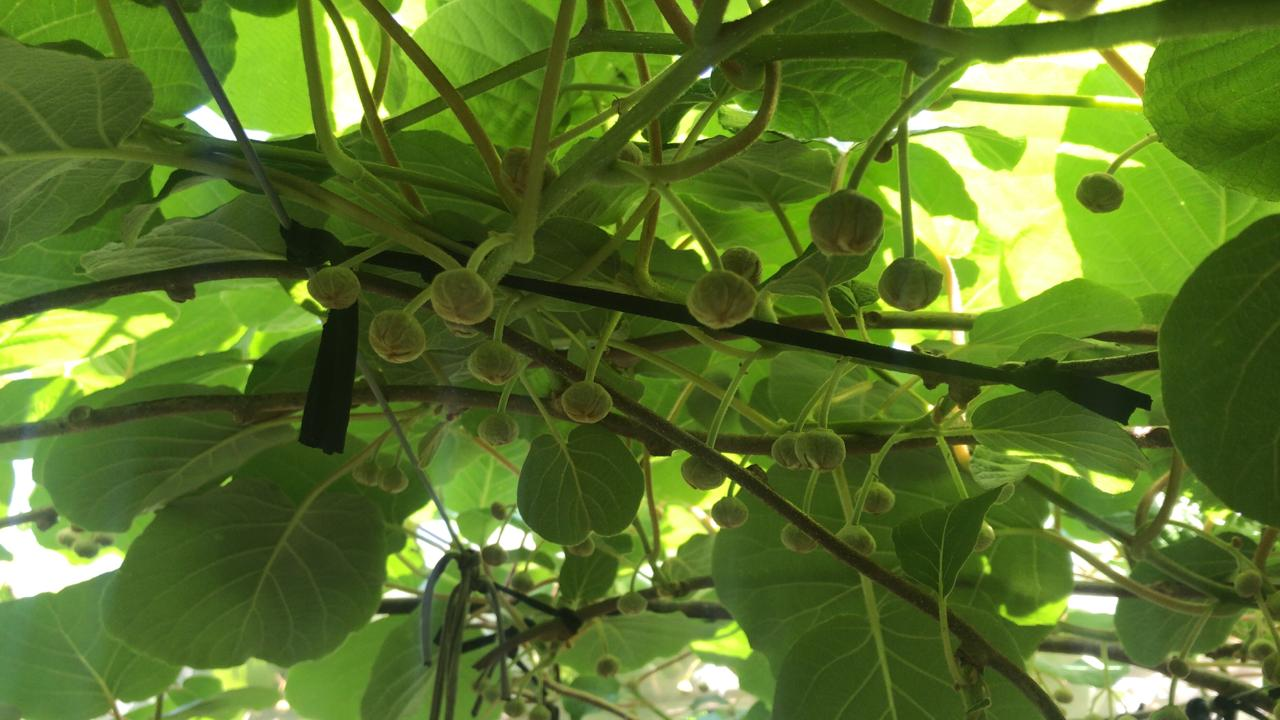
\includegraphics[width=.80\textwidth]{./Figures/kiwi_samsung.jpg}
         \caption{Foto con cámara Samsung Wb550.}
         \label{fig:1de2}
     \end{subfigure}
     \hfill
     \begin{subfigure}[b]{1.0\textwidth}
         \centering
         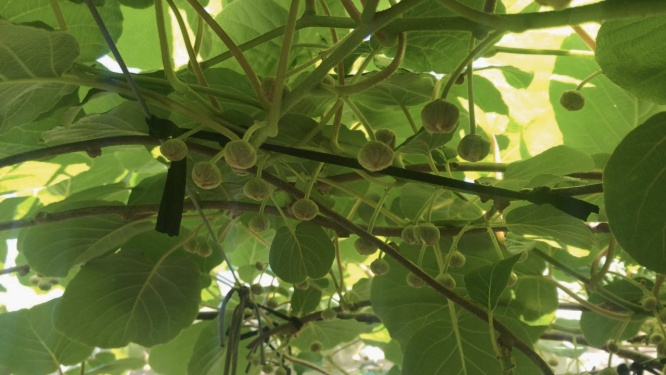
\includegraphics[width=.80\textwidth]{./Figures/kiwi_Ov7670.jpg}
         \caption{Foto con cámara Ov7670.}
         \label{fig:2de2}
     \end{subfigure}
     \hfill

        \caption{Comparación de capturas realizadas.}
        \label{fig:comparacion_fotos}
\end{figure}

\section{Pruebas de campo}
\label{pruebas_de_campo}

La realización de pruebas de campo constituye una etapa fundamental en la validación de sistemas destinados a operar en entornos reales. Sin embargo, en el contexto de este proyecto, la ejecución de pruebas de campo se tornó imposible debido a diversos factores logísticos y a la falta de disponibilidad de las cosechas necesarias para completar los ensayos.

La validación de sistemas en campo requiere acceso regular y continuo a las condiciones ambientales donde se prevé el uso final. En este caso, el sistema fue diseñado para monitorear cultivos de kiwi, lo que implicaba ensayos en un ambiente agrícola. Lamentablemente, la disponibilidad de las cosechas de kiwi se vio comprometida debido a condiciones ajenas al control del proyecto.

Esta imposibilidad de validar en el campo presenta desafíos para la evaluación final del sistema. Las pruebas de campo habrían permitido observar el rendimiento de cada módulo en condiciones de variabilidad ambiental, incluyendo factores como el cambio de luz, la humedad y las fluctuaciones en la temperatura, que afectan directamente la calidad de los datos capturados. Sin embargo, en ausencia de estos ensayos, la evaluación debió limitarse al entorno controlado de laboratorio, que, aunque útil, no permite replicar las condiciones exactas de operación en campo abierto. Esto limita parcialmente la verificación de la robustez del hardware y el firmware en situaciones reales. Aunque la falta de pruebas en campo representa una limitación en los resultados, la metodología utilizada y las pruebas en entorno controlado aportan una base sólida para futuras iteraciones del sistema.
 
	% Chapter Template

\chapter{Conclusiones} % Main chapter title

\label{Chapter5} % Change X to a consecutive number; for referencing this chapter elsewhere, use \ref{ChapterX}


%----------------------------------------------------------------------------------------

%----------------------------------------------------------------------------------------
%	SECTION 1
%----------------------------------------------------------------------------------------

\section{Conclusiones generales }

La idea de esta sección es resaltar cuáles son los principales aportes del trabajo realizado y cómo se podría continuar. Debe ser especialmente breve y concisa. Es buena idea usar un listado para enumerar los logros obtenidos.

Algunas preguntas que pueden servir para completar este capítulo:

\begin{itemize}
\item ¿Cuál es el grado de cumplimiento de los requerimientos?
\item ¿Cuán fielmente se puedo seguir la planificación original (cronograma incluido)?
\item ¿Se manifestó algunos de los riesgos identificados en la planificación? ¿Fue efectivo el plan de mitigación? ¿Se debió aplicar alguna otra acción no contemplada previamente?
\item Si se debieron hacer modificaciones a lo planificado ¿Cuáles fueron las causas y los efectos?
\item ¿Qué técnicas resultaron útiles para el desarrollo del proyecto y cuáles no tanto?
\end{itemize}


%----------------------------------------------------------------------------------------
%	SECTION 2
%----------------------------------------------------------------------------------------
\section{Próximos pasos}

Acá se indica cómo se podría continuar el trabajo más adelante.
 
\end{verbatim}

Los apéndices también deben escribirse en archivos .tex separados, que se deben ubicar dentro de la carpeta \emph{Appendices}. Los apéndices vienen comentados por defecto con el caracter \code{\%} y para incluirlos simplemente se debe eliminar dicho caracter.

Finalmente, se encuentra el código para incluir la bibliografía en el documento final.  Este código tampoco debe modificarse. La metodología para trabajar las referencias bibliográficas se desarrolla en la sección \ref{sec:biblio}.
%----------------------------------------------------------------------------------------

\section{Bibliografía}
\label{sec:biblio}

Las opciones de formato de la bibliografía se controlan a través del paquete de latex \option{biblatex} que se incluye en la memoria en el archivo memoria.tex.  Estas opciones determinan cómo se generan las citas bibliográficas en el cuerpo del documento y cómo se genera la bibliografía al final de la memoria.

En el preámbulo se puede encontrar el código que incluye el paquete biblatex, que no requiere ninguna modificación del usuario de la plantilla, y que contiene las siguientes opciones:

\begin{lstlisting}
\usepackage[backend=bibtex,
	natbib=true, 
	style=numeric, 
	sorting=none]
{biblatex}
\end{lstlisting}

En el archivo \file{reference.bib} se encuentran las referencias bibliográficas que se pueden citar en el documento.  Para incorporar una nueva cita al documento lo primero es agregarla en este archivo con todos los campos necesario.  Todas las entradas bibliográficas comienzan con $@$ y una palabra que define el formato de la entrada.  Para cada formato existen campos obligatorios que deben completarse. No importa el orden en que las entradas estén definidas en el archivo .bib.  Tampoco es importante el orden en que estén definidos los campos de una entrada bibliográfica. A continuación se muestran algunos ejemplos:

\begin{lstlisting}
@ARTICLE{ARTICLE:1,
    AUTHOR="John Doe",
    TITLE="Title",
    JOURNAL="Journal",
    YEAR="2017",
}
\end{lstlisting}


\begin{lstlisting}
@BOOK{BOOK:1,
    AUTHOR="John Doe",
    TITLE="The Book without Title",
    PUBLISHER="Dummy Publisher",
    YEAR="2100",
}
\end{lstlisting}


\begin{lstlisting}
@INBOOK{BOOK:2,
    AUTHOR="John Doe",
    TITLE="The Book without Title",
    PUBLISHER="Dummy Publisher",
    YEAR="2100",
    PAGES="100-200",
}
\end{lstlisting}


\begin{lstlisting}
@MISC{WEBSITE:1,
    HOWPUBLISHED = "\url{http://example.com}",
    AUTHOR = "Intel",
    TITLE = "Example Website",
    MONTH = "12",
    YEAR = "1988",
    URLDATE = {2012-11-26}
}
\end{lstlisting}

Se debe notar que los nombres \emph{ARTICLE:1}, \emph{BOOK:1}, \emph{BOOK:2} y \emph{WEBSITE:1} son nombres de fantasía que le sirve al autor del documento para identificar la entrada. En este sentido, se podrían reemplazar por cualquier otro nombre.  Tampoco es necesario poner : seguido de un número, en los ejemplos sólo se incluye como un posible estilo para identificar las entradas.

La entradas se citan en el documento con el comando: 

\begin{verbatim}
\citep{nombre_de_la_entrada}
\end{verbatim}

Y cuando se usan, se muestran así: \citep{ARTICLE:1}, \citep{BOOK:1}, \citep{BOOK:2}, \citep{WEBSITE:1}.  Notar cómo se conforma la sección Bibliografía al final del documento.

Finalmente y como se mencionó en la subsección \ref{subsec:configurando}, para actualizar las referencias bibliográficas tanto en la sección bibliografía como las citas en el cuerpo del documento, se deben ejecutar las herramientas de compilación PDFLaTeX, BibTeX, PDFLaTeX, PDFLaTeX, en ese orden.  Este procedimiento debería resolver cualquier mensaje "Citation xxxxx on page x undefined".
